\chapter{Structural Optimization}
\label{ch:struct_opt}

    \section{Introduction}
    
    The following chapter describes the various procedures used to determine an average description of the geometry of extra-framework water molecules as a function of fill. First, the volume of the supercell is optimized through a Birch-Murnaghan equation of state fitting in Section \ref{sec:eos}. Then, an assumption implemented in existing studies is tested in Section \ref{sec:da} (i.e. decoupling of the water molecule from the beryl framework) before internal relaxations of the supercell are carried out in various configurations in Section \ref{sec:geo_opt}.
    
    For each of the three sub-processes mentioned above, relevant background information, procedures, computational details, and analyses are provided. As each sub-process builds upon the previous' results, the final results and conclusions of this chapter are highlighted at the end of Section \ref{sec:geo_opt}.
    
    \section{Equation of State}
    \label{sec:eos}
        \subsection{Background Information}
        
            An equation of state describes the relationship between thermodynamic properties of a system. For instance, the Birch-Murnaghan equation of state, as described in detail in \textbf{[CITE: ((bmeos)) PRB 70,224107]},
            
            \begin{equation}
            \label{eq:bm_eos}
                E(\eta) = E_0 + \frac{9B_0V_0}{16}\left(\eta^2 -1\right)^2\left[ B'_0 \left(\eta^2-1\right) -4\eta^2\right] \text{ with } \eta = \left(\frac{V}{V_0}\right)^{1/2}
            \end{equation}
            
            \noindent relates the optimum volume $V_0$, the bulk modulus $B_0$, the first derivative of the bulk modulus $B'_0$, and the energy of the system $E$ as a function of current volume $v$. (Or, rather here, the normalized volume $\eta$ is used.)
            
            Equation \ref{eq:bm_eos} suggests a technique for determining the aforementioned thermodynamic quantities by calculating the energy of a system at various scaled volumes, which is outlined below.
        \subsection{Procedure}
        
        The following is a general procedure for fitting any equation of state, such as Eq. \ref{eq:bm_eos}. First, an initial "guess" structure $\sigma_g$ is acquired, typically from theory or experiment, with volume $V_g$. Using this structure, an ensemble of structures $\sigma_i$ with volume $V_i$ are constructed such that
        
        \begin{equation}
        \label{eq:ensem_eos}
            V_i \in \{ V_i : (1-x)V_g \le V_i \le (1+x) V_g \},
        \end{equation}
        
        \noindet for $x<1$. The initial structure $\sigma_g$ should be such that the set $\{V_i\}$ corresponds to volumes in neighborhood of $V_0$. Using each corresponding structure, the energy is calculated $E_i(V_i)$ via a self-consistent run. Finally, the resulting data is fit to Eq. \ref{eq:bm_eos} and the relevant optimized parameters are extracted.
        
        \subsection{Computational Details}
        
            For the beryl-water system, the set of $\{ V_i\}$ was sampled first in a course-grained manner with $8.7 \le a \le 9.6$ \angstrom  and $\Delta a = 0.1$ \angstrom. Then, a fine-grain scan is performed with $9.20 \le a \le 9.38$ \angstrom with $\Delta a=0.01$ \angstrom. Here, $a$ is the length of lattice vector $\Vec{a}$, which is related to the volume via
            
            \begin{equation}
                V(a) = \frac{\sqrt{3}}{2} a^2 c \text{ with } \frac{c}{a} = 0.998
            \end{equation}
            
            \noindent for beryl.
            
            The standard self-consistent calculator as outlined in \textbf{MAKE CALCULATOR SECTION} is employed for the self-consistent calculations. 
            
        \subsection{Results and Conclusions}
        
        \begin{figure}
            \centering
            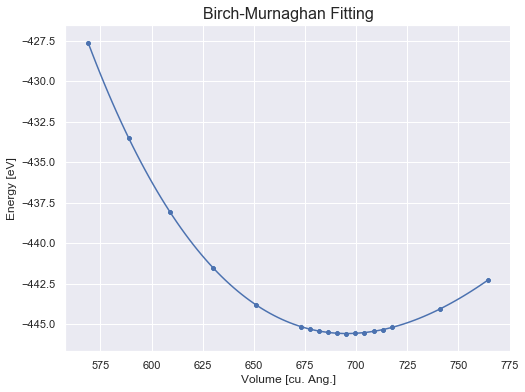
\includegraphics[width=0.8\linewidth]{Figures/System/eos.png}
            \caption{The calculated energies $E_i(V_i)$ are shown with the accompanying Birch-Murnaghan equation of state fit. The optimized volume is $V_0=695.50$ \angstrom$^3$. See text for literature comparison.}
            \label{fig:eos_fit}
        \end{figure}
        
        \begin{table}[]
            \centering
            \begin{tabular}{c|c|c}
                Observable & Value & Experiment \textbf{[CITE: eosfit]} \\
                \hline
                \hline
                $V_0$ [\angstrom$^3$] & 695.39 & $675\pm0.1$ \\
                $B_0$ [eV/\angstrom$^3$] & 1.1249 & $1.1 \pm 0.01$ \\
            \end{tabular}
            \caption{The optimized volume and bulk modulus as extracted from the fit in Fig. \ref{fig:eos_fit} are compared to literature values. See text for analysis.}
            \label{tab:eos_compare}
        \end{table}
        
        The results from the fitting are depicted in Fig. \ref{fig:eos_fit} and compared to literature values in Table \ref{tab:eos_compare}. The calculated optimized volume of $V_0 = 695.39$ \angstrom$^3$ is in good agreement with the literature value of $V=675\pm0.1$ \angstrom$^3$, especially considering that the literature values are determined at ambient temperature and pressure. 
        
        Moving forward, the cell volume will be fixed to $V=695.39$ \angstrom$^3$.
    \section{Decoupling Assumption}
    \label{sec:da}
        \subsection{Background Information}
            As previous work has demonstrated, there is no appreciable difference in geometry, potential map, or vibrational frequencies in terms of different exchange-correlation functionals, both with and without dispersion corrections \cite{vibr_states}. Effectively, this allows the crystal framework to be viewed as producing a static potential well in which the extra-framework water molecules interact. While this assumption is definitely ideal in terms of computational cost due to the relatively large number of ions and electrons in the beryl unit cell, this assumption needs to be explicitly tested before performing the geometry optimization.
            
            To this end, in the following the results of relaxing the full crystal-water system are compared to those obtained when the beryl framework is held fixed and only the water molecule is allowed to relax. Additionally, two different energy difference tolerances for self-consistency are tested.
        \subsection{Procedure}
            To begin, a single water molecule is added to the unit cell of beryl in the standard position. Such a system has a fill factor of 50\%. For each energy difference tolerances, positional degrees of freedom for both beryl and the water molecule are allowed to relax---this is referred to as the \textit{full} relaxation. Then, the beryl ions are held fixed, and only the water molecule ions are allowed to relax---this is referred to as the \textit{selective} relaxation.
            
            To compare the two relaxation schemes, the difference in position of each ion between the full and selective relaxations are calculated. By looking at both the average displacement and the maximum displacement between ions, the validity of the decoupling assumption can be determined. Additionally, the average of the water molecule bond lengths and the OHO-angle are compared for both schemes. Again, assuming the decoupling assumption holds, there should be no appreciable difference in the geometry parameters of the water molecule.
        \subsection{Computational Details}
            For both the full and selective relaxation, the relaxation calculator is used. The relaxations are performed with EDIFF set to $10^{-4}$ and $10^{-5}$. After both relaxations have been performed for each energy difference tolerance, the Atomic Simulations Environment \textbf{[CITATION]} is used to calculate the difference in ionic positions for each atom $\Delta r_i$. From the set of all ionic position differences $\{\Delta r_i \}$, the average displacement $\langle \Delta r \rangle$ and maximum displacement $\Delta r_\text{max}$ are determined. Additionally, the average of the two OH bond lengths $\langle r_\text{OH} \rangle$ and the OHO angle $\theta$ are determined for both relaxation schemes.
            
            To test the convergence of the calculations, the ratios of the water geometry parameters for each energy difference tolerance are calculated, with a ratio near unity indicating that there is no significant difference with respect to the energy difference tolerances. Finally, the ratios of the average OH bond and OHO angle for the full and selective relaxations are compared, again with a ratio near unity indicating that the decoupling assumption holds.
        \subsection{Results and Conclusions}
        
        \begin{figure}
             \centering
             \begin{subfigure}[t]{0.45\textwidth}
                 \centering
                 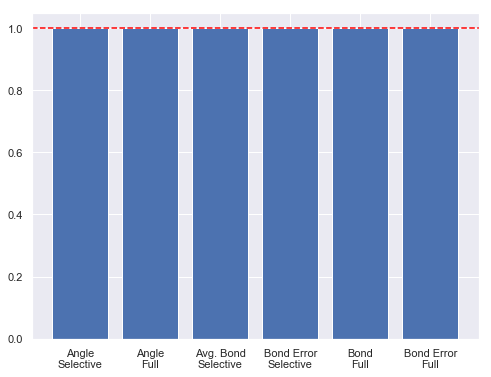
\includegraphics[width=\textwidth]{Figures/System/ediff_geom_ratios.png}
                 
                 \label{fig:ediff_geom_ratios}
             \end{subfigure}
             \hfill
             \begin{subfigure}[t]{0.45\textwidth}
                 \centering
                 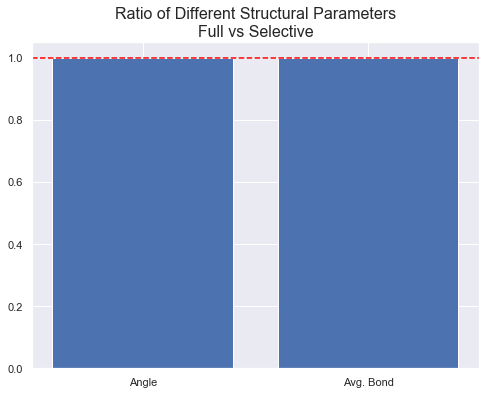
\includegraphics[width=\textwidth]{Figures/System/selective_v_full_geom_params.png}
                 \label{fig:selective_v_full}
             \end{subfigure}
                \caption{Decoupling assumption results. The red, dashed line denotes unity. (Left) The ratio of certain geometry parameters (and associated errors where appropriate) as calculated under energy difference tolerances $10^{-4}$ and $10^{-5}$. (Right) The ratio of OHO angle and average of the two OH bond lengths for the water molecule under the full and selective relaxation schemes with energy difference tolerance of $10^{-4}$. See text for full analysis.}
                \label{fig:decouple_assumption}
        \end{figure}
        
        The decoupling assumption results are summarized in Fig. \ref{fig:decouple_assumption}. Starting with the left sub-figure therein, it is clear that there is no measurable difference between the relevant geometry parameters in terms of energy stopping tolerance. Specifically, each observables ratio is nearly unity. It is therefore reasonable to conclude that the larger energy difference tolerance of $10^{-4}$ is suitable to use moving forward.
        
        \begin{table}[]
            \centering
            \begin{tabular}{c|c|c}
               Tolerance  & $\langle \Delta r \rangle$ & $\Delta r_\text{max}$  \\
               \hline
               \hline
                $10^{-4}$ & $0.008\pm 0.001$ & $0.031$  \\ 
                $10^{-5}$ & $0.010\pm0.001$& $0.033$ \\ 
            \end{tabular}
            \caption{The average difference in position over each ion and maximum difference in position between the two relaxation schemes for different energy difference tolerances. All distance measurements are in Angstroms.}
            \label{tab:ediff_r_diff}
        \end{table}
        
        Finally, to test the decoupling assumption the average OH bond length and OHO angle for both the full and selective relaxations with energy difference tolerance $10^{-4}$ are compared via their ratios in Fig. \ref{fig:decouple_assumption} (right). Again, both geometry parameters are nearly unity, suggesting there is no significant difference in the water molecule geometry between the two relaxation schemes. Furthermore, as shown in Table \ref{tab:ediff_r_diff}, both the average displacement and maximum displacement of the ions under the two relaxation schemes is significantly small compared to the length of the lattice vectors ($<1\%$ in both cases). 
        
        Therefore, the validity of the decoupling assumption is affirmed and will be implemented for the remainder of the study.
    \section{Geometry Optimization}
    \label{sec:geo_opt}
    
    With the validity of the decoupling assumption, and corresponding selective relaxation scheme, the geometry of the water molecules can be determined as a function of fill and rotation. Specifically of interest are the OH bond length and OHO angle and how they change when rotated about the high symmetry point of the beryl cage. Does these geometric parameters have a well-defined, meaningful average value? How do these parameters vary when the relative angle between extra-framework water molecules change? The remainder of this chapter sets out to answer those questions.
    
        \subsection{Procedure}
        
        \begin{figure}
            \centering
            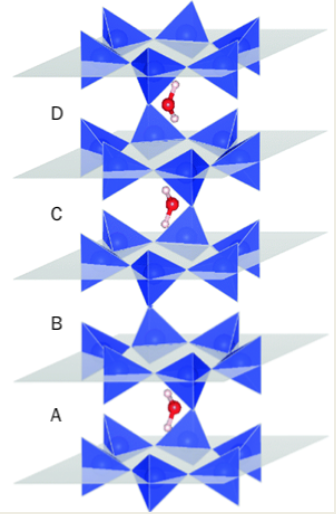
\includegraphics{Figures/System/geometry_supercell.png}
            \caption{Depiction of the supercell, with labeled cages A-D, used for the geometry optimization as outlined in the text. [\textbf{Adapted from 10.1039/c7cp06472a}]}
            \label{fig:geom_supercell}
        \end{figure}
        
        To start, a supercell is created by replicating the unit cell once in the c-direction, resulting in four cages, as shown in Fig. \ref{fig:geom_supercell}. The cages are labelled, starting from the bottom-most, as A, B, C, and D. With four cages, it is possible to probe fill factor $\phi \in \{0.25,0.50,0.75,1.00 \}$. For $\phi=0.50$, there exists a degeneracy in the fills, i.e. both configurations with A \& C filled and A \& B filled correspond to the same fill factor. To make discussion herein as unambiguous as possible, the binary conventions in Table \ref{tab:fill_conventions} are used throughout. Occasionally, the water molecule that occupies a cage may be referred to by the cage label. For example, in Fig, \ref{fig:geom_supercell}, the water molecule in cage C may be referred to as water molecule C. 
        
        \begin{table}[]
            \centering
            \begin{tabular}{c|c}
               Fill  & Occupied Cages \\
               \hline
               \hline
               1000  &  A \\
               1010  &  A, C \\
               1100  &  A, B \\
               1110  &  A, B, C \\
               1111  &  A, B, C, D\\
            \end{tabular}
            \caption{The binary convention adopted to describe the different fill possibilities.}
            \label{tab:fill_conventions}
        \end{table}
        
        While the fill factor $\phi$ provides one dimension of the parameter space to explore, it does not encompass the entirety of the space. The geometry must also be probed as a function of relative angle to the beryl framework \textit{and} the relative angle between water molecules. Naturally, only a smaller subspace of this parameter space can be sampled, and said subspace is outlined in Table \ref{tab:param_subspace}.
        
        For example, for fill 1110, molecule C is held fix, while molecule A is rotated through 12 rotations totaling $2\pi$, and for each rotation of A, molecule B is also rotates through 12 rotations totaling $2\pi$. In all, $12^2 = 144$ configurations are sampled for this fill. Also, for fill 1111, molecules A-C and B-D are pairwise ferroelectrically coupled, and therefore rotate together. 
        
        The above demonstrates the difficulty of adequately sampling this parameter space, especially considering the expense of these calculations (approximately 8 hours per configuration running on 16 cores). Given more resources, a greater sample size would be ideal, specifically increasing the number of rotations. It may also help optimization if the rotation angle were decreased to encompass only the asymmetric unit of the crystal.
        
        In addition to performing the above procedure with the water molecules in the beryl framework, the same is carried out on water molecules in the same configurations in the absence of the beryl crystal. In other words, the spacing and rotation of the water molecules is the same, but the calculations are carried out in vacuum. This allows for investigation of how the beryl framework affects the geometry, if at all.
        
        \begin{table}[]
            \centering
            \begin{tabular}{c|c|c|c}
                Fill & No. Rotations & Rotation Angle  & Rotated Molecules  \\
                \hline
                \hline
                1000 & 30 & $2\pi$ & A \\
                1010 & 12 & $2\pi$ & A, C \\
                1100 & 12 & $2\pi$ & A, B \\
                1110 & 12 & $2\pi$ & A, B \\
                1111 & 12 & $2\pi$ & A-C,B-D \\
            \end{tabular}
            \caption{Outline of the parameter subspace sampled as part of the geometry optimization. See text for details.}
            \label{tab:param_subspace}
        \end{table}
        
        \subsection{Computational Details}
        
        For each configuration in Table \ref{tab:param_subspace}, the selective relaxation scheme as outlined in \ref{sec:da} is used. After the relaxation, the relevant geometric measurements are made using ASE. 
        
        \subsection{Results and Conclusions}
        \label{sec:geom_opt}
        
        \begin{figure}
            \centering
            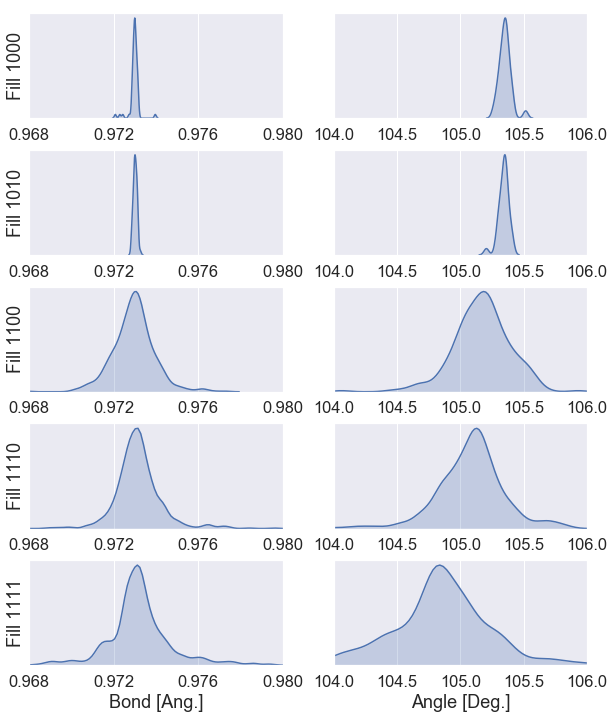
\includegraphics[width=0.85\linewidth]{Figures/System/geom_kdes.png}
            \caption{Kernel density estimates for the OH bond lengths (left) and OHO angles (angles) by fill. }
            \label{fig:geom_kdes}
        \end{figure}
        
        Figure \ref{fig:geom_kdes} shows the kernel density estimates for the OH bond lengths and OHO angles. Each subplot represents the population density of the sampled set. Immediately clear is the fact that there is an effect of fill on the geometry of the water molecules, as evident by the qualitative difference in shape of the population densities. In any case, for each, there is a well-defined peak, suggesting that an average geometry per fill is meaningful. However, the variance of the population density is directly proportional to the fill, suggesting that rotation does have some effect on the geometry. 
        
        
        
        \begin{figure}
            \centering
            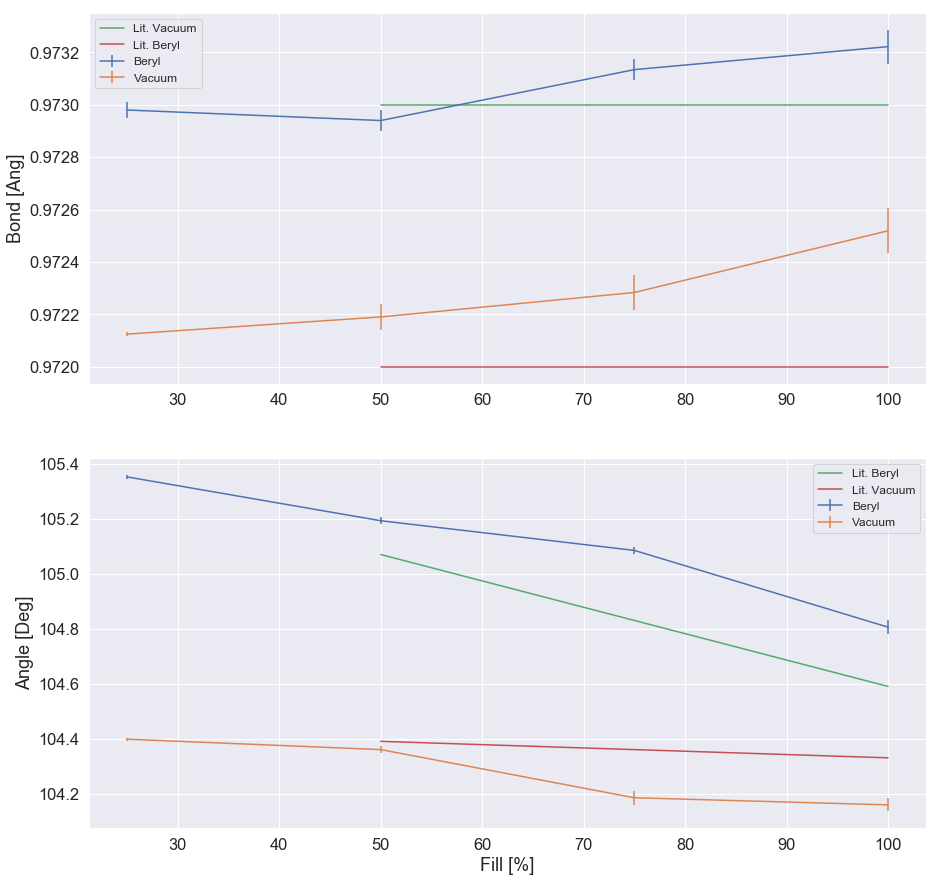
\includegraphics[width=0.85\linewidth]{Figures/System/geom_results.png}
            \caption{The average OH bond length (top) and OHO angle (bottom) per fill factor are compared to literature values, when possible. Error bars represent the standard errors of the mean.}
            \label{fig:geom_results}
        \end{figure}
        
        For a more quantitative analysis, the averages and standard errors of the mean are used as shown in Fig. \ref{fig:geom_results}. Here, the populations (and therefore, results) for fills 1010 and 1100 are combined. 
        
        From both the OH bond length and OHO bond angle (blue line), it is clear that there is an effect from the fill factor on the geometry of the water molecule. Specifically, as more water molecules are added, the OH bond lengthens slightly, while the OHO angle decreases. Additionally, an effect from the beryl crystal is evident (orange vs. blue line) in that the beryl has a \textit{dilating} influence on the water molecule---the OH bond length systematically increases and the OHO angle systematically expands. 
        
        As a benchmark, these results are acceptably compared to the work done in \cite{vibr_states} (green and red lines). Here, the systematic differences can be explained by the procedure followed in said work. Instead of relaxing the water molecule under the optimized beryl geometry, the beryl geometry was set to match an experimental sample to which they were comparing their computational results. Additionally, only fill factors $\phi = 0.50, 1.00$ were investigated. 
        
        Moving forward, the fill specific geometries, as shown in Fig. \ref{fig:geom_results}, are used. 
        
        \paragraph{Outlook}
        To improve upon these parameters, a larger subspace of the parameter space should be investigated. Additionally, changing the size and shape of the unit cell---and thus the fill configurations that correspond to certain fill factors $\phi$---and investigating the average geometry would be of interest as well. Notebly, what happens if the supercell is created by replicating the unit cell along the a- or b-directions? 